\chapter{Pilotage de la qualité}

% 
% Changer cette partie, pour la mettre dans une partie dédiée. 

\section{Dette technique}
La dette technique, est un concept reprenant le principe de la dette appliqué au domaine du développement logiciel.

\subsection{Présentation}

Un projet de développement d'une application inclut une conception logicielle (qu'elle soit formalisée ou pas).

Cette dernière fait partie de la qualité du projet. Écrire le code source en suivant la conception définie en amont lui permet d'être cohérent et de faciliter la maintenance :

\begin{itemize}
\item maintenance corrective : corriger les bug informatiques
\item maintenance évolutive : ajouter de nouvelles fonctionnalités au logiciel. 
\end{itemize}

Ainsi, un non-respect de la conception, intentionnel ou non, induit des coûts supplémentaires dans le futur. 
Ce sont les intérêts. C'est pourquoi l'on parle de dette technique, pour montrer l'analogie avec la dette dans les finances des entreprises. 
Cela sous entend qu'il vaut mieux rembourser la dette un jour plutôt que de continuer à payer sans cesse des intérêts.
\jumpTwo
En résumé, quand on code au plus vite et de manière non optimale, on contracte une dette technique que l'on rembourse tout au long de la vie du projet sous forme de temps de développement de plus en plus long et de bugs de plus en plus fréquents.

Selon le rôle que l’on joue dans le projet, la perception que l’on en a varie du tout au tout.

\paragraph{Exemple :} Le client peut mettre la pression pour que le projet sorte rapidement sans comprendre les enjeux techniques, le développeur sous-traitant en retard ne souhaite qu’une chose : en finir avec ce projet, le repreneur du projet se demande ce qu’il va pouvoir faire avec cette horreur après un audit.

Dans un projet, la qualité augmente la charge de travail, ce qui peut avoir un impact sur le délai immédiat. Ainsi, lors de la survenue imminente d'une nouvelle version du logiciel, respecter la conception idéale peut mettre en péril la livraison d'une nouvelle version du logiciel. 
À ce moment précis, ne pas respecter la conception idéale peut permettre d'atteindre l'objectif prioritaire à court terme (sortir une nouvelle version) mais augmente considérablement la dette technique. 

\subsection{Typologie}

\subsubsection{Dette involontaire}
Elle résulte d’un mauvais choix technique de n’importe quel ordre (ergonomique, algorithmique, stratégique, etc.). Ses sources sont multiples : mauvais choix du framework, redondance de code, script copié/collé depuis un forum, etc. Le manque de connaissances (technique ou métier) ou la mauvaise communication au sein d’une équipe en sont les causes plus répandues.

\subsubsection{Dette volontaire non assumée}
Elle résulte d’une décision technique pris en connaissance de cause mais dont le choix ou la mise en œuvre sont perfectibles. Les intervenants se renvoient la “patate chaude” au moment de l’apparition des problèmes dont on repousse la résolution à “plus tard”. Cette dette est la plus courante et est souvent due aux délais de réalisation très courts des projets, dans un périmètre fonctionnel rarement fixé au préalable.

\subsubsection{Dette volontaire assumée}
Résulte de tous les choix techniques n’appartenant pas aux deux premiers types de dette. En effet, tout choix implique des conséquences, et ce qui peut paraître la meilleure option à l’instant T, ne le sera peut-être plus à T+1, voir T+10, et il faudra malgré tout faire avec.
\jumpOne

\subsection{Bob Booking}
Lorsque l'application Bob Booking a été développée, les phases de qualité et particulierement celles de rédaction de tests unitaires, tests d'intégration et fonctionnel ont été volontairement mise de coté au profit d'un temps de développement plus court pour sortir l'application plus rapidement. 

8 ans après le développement de Bob Booking, l'équipe technique paye au prix fort le poids de la dette technique : 

\subsubsection{Effets}

\begin{description}
    \item L'implémentation de nouvelles fonctionnalités est de plus en plus long 
    \item L'application contient de plus en plus d'effets de bord indésirables, rendant la maintenance corrective trop importante pour un projet de cette envergure. 
    \item A chaque nouvelle fonctionnalité développée, l'aspect qualité est volontairement mis de coté. Ainsi chaque nouveau développement accroit le poids de la dette, enfermant l'équipe de développement dans un cercle vicieux. 
    \item La non-documentation de l'application Bob Booking augmente considérablement le temps de formation d'un nouveau développeur sur l'application. 
    Toute nouvelle personne travaillant sur Bob Booking, ne pourra pas être autonome rapidement et devra questionner de manière récurrente l'équipe de développement pour comprendre le fonctionnement de l'application. \\
    L'entreprise perd donc beaucoup de temps à former les nouvelles personnes sur Bob Booking et par conséquent perd également de l'argent. 
\end{description}

\begin{figure}[h!]
\centering
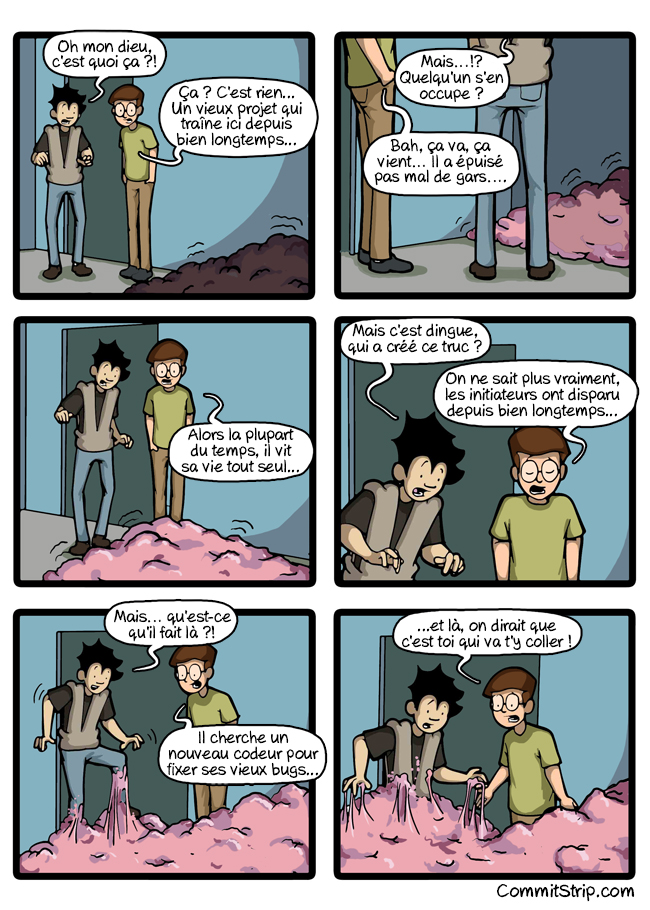
\includegraphics[width=0.45\textwidth]{assets/blob.jpg}
\caption{Illustration de la dette technique}
\label{fig:my_label}
\end{figure}

\newpage

\section{Pourquoi le pilotage de la qualité}

Plus que jamais, s’appuyer sur des infrastructures informatiques pérennes et robustes constitue un élément stratégique pour les entreprises. 
On constate pourtant que beaucoup d’entreprises déplorent une qualité médiocre des développements réalisés et investissent des sommes considérables pour pallier à cette problématique. Ce constat est particulièrement évident lorsque qu’il s’agit d’une application stratégique, pouvant impacter fortement les performances ou la qualité de service d’une entreprise.


\subsection{La théorie}

Le pilotage de la qualité est un aspect incontournable du développement. 
C'est un processus complexe qui doit être mené dès le début du cycle de développement du projet afin de porter ses fruits. 

Le pilotage de la qualité doit prendre en considération plusieurs paramètres pour être efficace : 

\begin{description}
\item[Paramètres technologiques]{où le logiciel doit être maintenable, fiable, évolutif, sécurisé,
transferable proposant ainsi une infrastructure informatique pérenne et robuste.} 
\item[Paramètres organisationnels]{et relatif à la gestion de projet, permettant d'appliquer les bonnes pratiques tout au long du développement du logiciel.} 
\end{description}

\newpage

Lorsque ces deux aspects sont en synergie, ils permettent de garantir un pilotage efficace. 
En effectuant une conduite de la qualité de manière continue cela permet de prévenir beaucoup d'erreurs en amont de la sortie du logiciel et permettre de limiter l'impact technique et financier. 
De manière plus générale, cet aspect qualitatif, doit permettre aux entreprises de structurer leur approche du développement en mettant en place des règles strictes pour tout nouveau projet. 

Le pilotage de la qualité doit également être intuitif et lisible par les différentes populations de l'entreprise et ne doit donc pas être uniquement réservé aux développeurs. 
A l'aide de tableaux de bords proposant une vision claire et précise du projet pour permettre alors de partager la situation avec tous les acteurs du projet. 

\section{Pilotage de la qualité dans la pratique}

Le paragraphe précédent, aborde le pilotage de la qualité d'un point de vue théorique, mais comment mettre en place ces préceptes de manière simple et efficace dans la pratique?

\section{Conception}

La phase de conception du logiciel est tout aussi importante voir même plus importante que la phase d'écriture du code. 
Les développeurs se doivent de réfléchir à tous les aspects du logiciel en amont. 
Plusieurs méthodes permettent d'être efficace sur ce point. 

\subsubsection{User story}
Les user story ou récit d'utilisateur en français sont des phrases simple dans le langage naturel permettant de décrire avec suffisamment de précision le contenu d'une fonctionnalité à développer. 

La phrase contient généralement trois élements descriptifs de la fonctionnalité : Qui ? Quoi ? Pourquoi ? 

\paragraph{Exemple}

\begin{verbatim}
En tant qu'utilisateur
je veux pouvoir rechercher mes clients par leur prénom et leur nom de famille afin de les
retrouver rapidements lorque je reçois un appel de leur part. 

En tant qu'utilisateur,
je veux pouvoir modifier mes emplois du temps mais pas ceux des autres utilisateurs
\end{verbatim}

\subsubsection{Use case}
Les use cases ou cas d'utilisation, représente une interaction possible entre un utilisateur et le système. 

La rédaction des cas d'utilisations passe par des diagrammes d'utilisation. 

Les utilisateurs sont appelés acteurs et ils interagissent dans les cas d'utilisations.


\begin{figure}[h!]
\centering
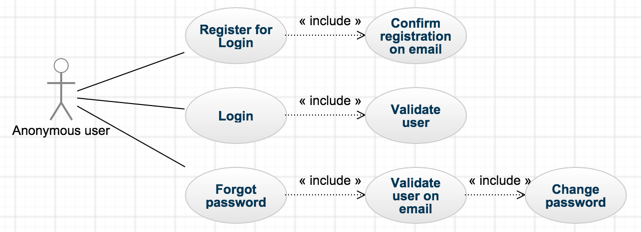
\includegraphics[width=1\textwidth]{assets/use_case_exemple.png}
\caption{Exemple d'un diagramme de cas d'utilisation}
\label{fig:my_label}
\end{figure}

\newpage

\subsubsection{Diagramme d'activité}

Permettant de représenter le déclenchement d'événements en fonction des états du système.
Il peut être également utilisé pour décrire un flux de travail. 

\begin{figure}[h!]
\centering
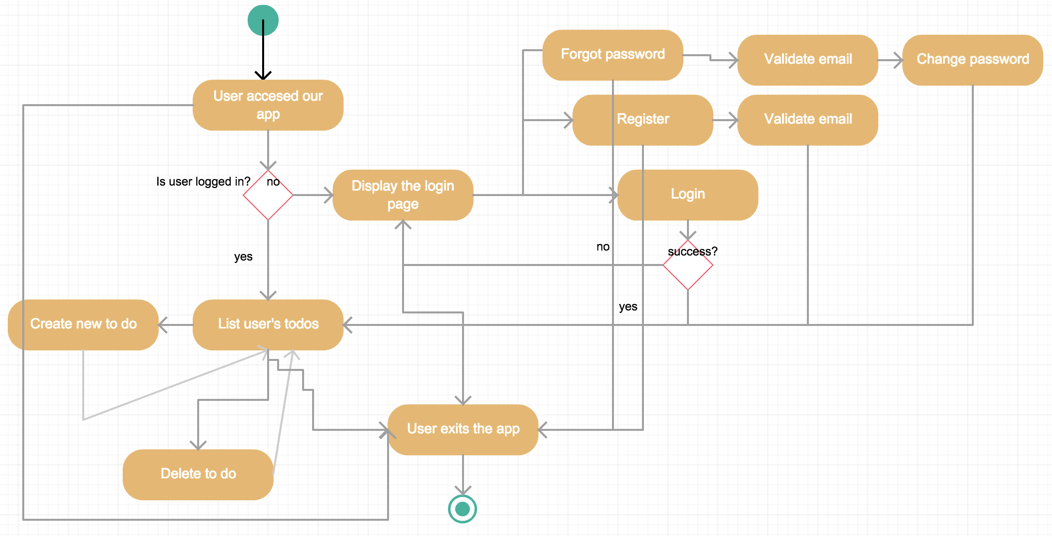
\includegraphics[width=1\textwidth]{assets/activity_diagram.png}
\caption{Exemple d'un diagramme de cas d'utilisation pour un gestionnaire des tâches}
\label{fig:my_label}
\end{figure}

Ce diagramme sera particulièrement utile pour définir les différents chemins qu'un utilisateur peut prendre dans notre application et donc définir ceux qu'ils ne peut pas prendre et mettre en place les routines de sécurité en conséquence. 

\paragraph{Exemple des activités exprimées dans le diagramme ci-dessus}
\begin{verbatim}
- Un utilisateur accede à notre gestionnaire des tâches 
- Si l'utilisateur n'est pas connecté, il verra la page de connection.
- Si l'utilisateur a déjà un compte, il peut se connecter
- Si l'utilisateur a un compte mais a oublié son mot de passe, il peut récupérer son mot de passe
- Si l'utilisateur n'a pas de compte, il peut en créer un. 
- Les deux actions, créer un compte et récupérer mon mot de passe nécessitent une validation d'email. Un utilisateur peut se connecter à l'application, uniquement après que son adresse email ait été confirmé. 
- Si l'utilisateur est déjà connecté, il verra son gestionnaire des tâches (qui peut être vide si il ne contient pas de tâches). 
- Lorsqu'il est connecté l'utilisateur peut 
  - voir sa liste des tâches
  - marquer une tâche comme effectuée
  - rechercher dans sa liste des tâches
  - supprimer une tâche d'une liste
  - se déconnecter
- L'utilisateur peut se déconnecter à tout moment 
\end{verbatim}



\section{Tests}
Un test désigne une procédure permettant de vérifier partiellement un système. 

\subsubsection{Objectif}
L'objectif premier des tests est d'identifier les comportements problématiques du logiciel pour en augmenter la qualité. 

\subsubsection{Classification des tests}

\begin{figure}[h!]
\centering
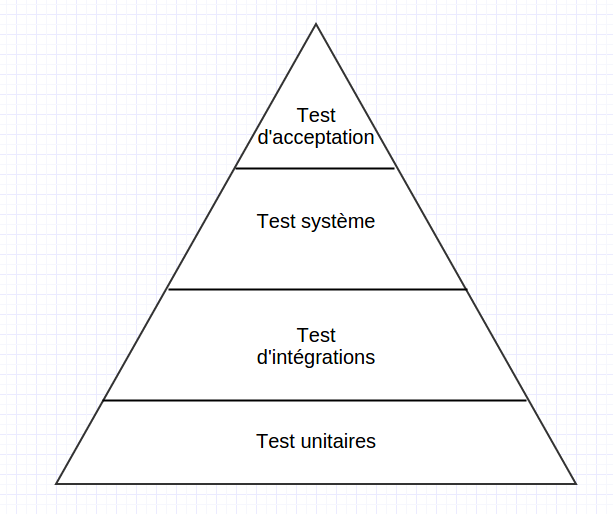
\includegraphics[width=0.7\textwidth]{assets/pyramide_tests.png}
\caption{Quatres niveaux de test}
\label{fig:my_label}
\end{figure}

Chaque test supérieur, dépend du test de niveau inférieur. 
Ainsi si les tests d'intégration ne fonctionnent pas, les tests système ne s'executeront pas. 


\subsection{Test unitaires}
Les tests unitaires sont des procédures permettant de vérifier le bon fonctionnement d'une partie précise d'un logiciel ou d'un module d'un programme. 

\subsubsection{Utilité}
Ils permettent d'assurer que la spécification correspondante à la partie du logiciel testée est bel est bien réalisée. 


\begin{description}
    \item Ils permettent également de trouver rapidement les erreurs 
    \item Ils permettent également de sécuriser la maintenance en signalent les éventuelles régressions du programme, en cas de modification. Certains tests peuvent échouer lorsqu'une nouvelle fonctionnalité est implémentée, il faut donc réécrire le test pour le faire correspondre aux nouvelles attentes, ou corriger l'erreur dans le code. 
    \item Les tests unitaires permettant enfin de documenter le code. En lisant un test unitaire, on va pouvoir comprendre très rapidement le fonctionnement d'une méthode. Il est possible que la documentation d'une application ne soit plus à jour, en revanche les tests eux correspondent à la réalité de l'application. 
\end{description}

Les tests unitaires sont aussi simples que possible, facilement "débugable", doivent être rapides à éxecuter

Voir l'annexe, pour un exemple de test unitaire. 
% Annexe emple de test unitaire


\subsection{Test d'intégration}
Les tests d'intégration chacun des modules indépendants du logiciel sont assemblés et testés dans l'ensemble. 

\subsubsection{Objectifs}
L'objectif est de détecter les erreurs qui n'ont pas pu être détectées lors des tests unitaires. 

Ces tests permettent également de vérifier l'aspect fonctionnel du logiciel ainsi que ses performances et sa fiabilité. 

La particularité des tests d'intégration est l'environnement.
En effet, les tests unitaires vont être executés dans l'ensemble effectuant différentes actions (requêter une base de donnée, consumer un service REST, etc), et ceux dans différents environnement pour s'assurer que les différents environnement n'affectent pas le comportement du code. 

\subsection{Test système}
Les test système permettent d'évaluer la conformité du système face aux exigences spécifiées.

Ces tests vérifient la conception mais également le comportement et les attentes présumées du client. 


\subsection{Test d'acceptation}
C'est le dernier niveau de test, on l'appelle également recette. 

Ce test vise à assurer de manière formelle que le produit complet est conforme aux spécifications. 

\paragraph{Exemple de tests d'acceptation}

\begin{verbatim}
- Cliquer sur le bouton de zoom, doit élargir le document de 25%
\end{verbatim}

L'avantage de ces tests et qu'ils sont écrit en langage naturel (français par exemple) et s'assure que l'ensemble des fonctionnalités du logiciel fonctionne. 
Cependant les tests d'acceptation peuvent s'avérer particulièrement difficile à débuger, car ils se basent sur beaucoup de lignes de code. 

Egalement, en méthodologie agile, les test d'acceptation sont censés être le miroir des user stories (vu précédemment). 
Si les tests passent, ça signifie que la user story rejoint les besoins du client et que cette récit utilisateur est complet. 

% Ajouter la documentation. 

\subsubsection{Conclusion}

Tous ces tests sont complémentaires. Parfois il est préférable de se concentrer sur un type de test ou d'en éviter d'autres.
La principale différence entre ces différents niveaux de test, réside dans le fait que certains tests sont destinés au développeur, tandis que d'autres aux attentes clients. 

\section{Usine logiciel}
L'intégration d'un projet est constituée de différentes étapes souvent laborieuses et consommatrices de temps. Parmi ces étapes, nous retrouvons généralement les phases de génération de code, de compilation, l'exécution d'outils de qualité de code, l'exécution d'outils de tests unitaires et fonctionnels, de génération de code, des phases de validation et de vérification d'éléments transverses comme les licences, de déploiement, ...
\jumpOne
Cette phase d'intégration est d'autant plus critique qu'elle est faite en fin de projet avant la livraison, et que révélant de nombreux problèmes elle risque de mettre la réussite du projet en péril.
\jumpOne
L'ensemble de ces problèmes sont supprimés avec la mise en place de l'intégration continue qui va constiter à mettre en place un ensemble d'outils pour automatiser le processus d'intégration. Celui-ci est exécuté à chaque changement dans l'environnement d'infrastructure du projet et produit un ensemble de résultats que les membres de l'équipe de développement puissent visualiser à chaque instant.

\subsection{Intégration continue}
L'intégration continue est une pratique visant à vérifier qu'à chaque modification du code d'un logiciel, il ne se produit pas de régression sur ce logiciel. 

L'intégration est utilisée à l'aide d'une plateforme d'intégration continue (comme Jenkins).

Cette plateforme va permettre aux développeurs de pouvoir déployer leurs applications, d'une manière automatisée et industrielle en validant un certain nombre de règles que le projet doit respecter pour être mis en production.
\jumpOne
A chaque modification du code (généralement provoqué par un \gls{commit}
d'un des developpeurs, un processus est lancé et va executer tous les tests unitaires et fonctionnels. 
En plus d'éxecuter les tests, généralement une analyse statique du code est effectuée, permet de déterminer la qualité du code en lui même. 

\begin{itemize}
\item Détection rapide d'une anomalie logicielle et diminution du coût tardif d'une correction logicielle
\item Cohésion de l'équipe de développement
\item Automatisation des tests
\item Suivi de la qualité du code logiciel
\item Visibilité dans l'avancement du projet
\item Version déployée et disponible en continue
\item Automatisation de la livraison
\end{itemize}

\begin{figure}[h!]
\centering
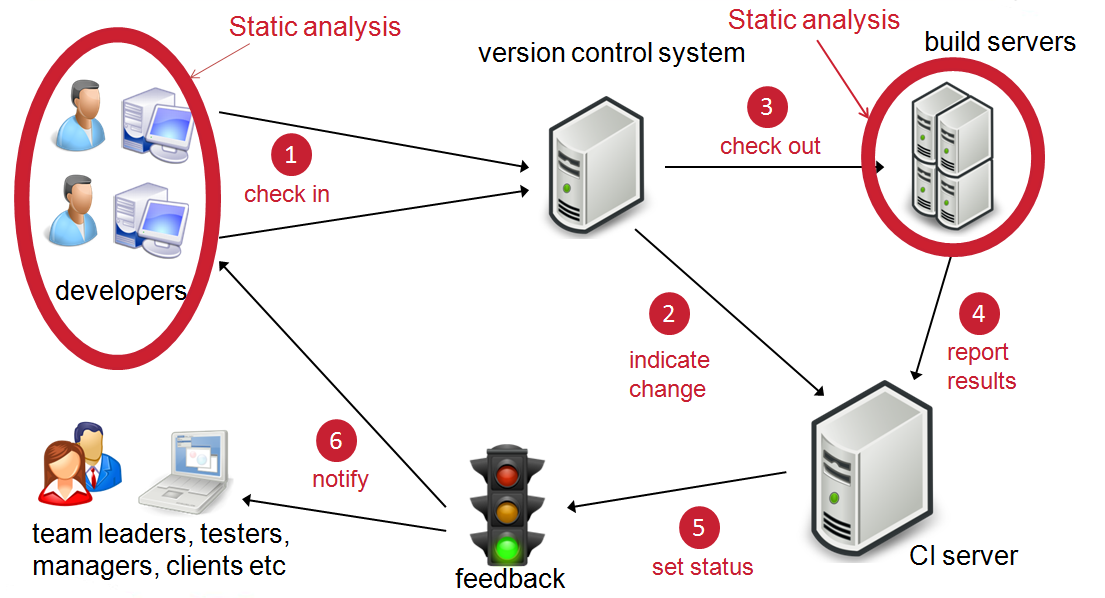
\includegraphics[width=0.7\textwidth]{assets/ci.png}
\caption{Intégration continue}
\label{fig:my_label}
\end{figure}

\paragraph{Explication}
\begin{enumerate}
\item Les développeurs publient leurs modifications au système de versionning
\item Ce système indique au gestionnaire d'intégration continue un chargement
\item Les tests sont exécutés ainsi que l'analyse statique du code
\item Le serveur d'intégration continue rapporte par la suite aux développeurs et au management l'état du projet après les modifications.
\end{enumerate}

\section{Revue de code}
La revue de code est un autre moyen d'identifier des bugs. 
Il consiste à faire une revue du code source développée par un développeur expérimenté. 

La mise en place de revue de code, de manière systématique pendant la phase de développement permet de responsabiliser les développeurs car, le travail de chacun sera systématiquement évalué par quelqu'un d'autre. 

Ce système va permettre d'améliorer la qualité du code écrit. De plus le relecteur pourra identifier des bugs ou des axes d'amélioration possible. 

Il existe trois processus de revue de code 

\begin{enumerate}
    \item Revue de code bloquante : Tout développement doit être relu avant d'être commité sur le \gls{depot} 
    A comme inconvénient de freiner le développement, car certains développements peuvent se retrouver en attente d'une relecture dont ils dépendent. 
    \item Revue de code non-bloquante : Tout développement commité sur le dépôt doit être relu. 
    Permet de laisser les développeurs continuer à travailler sans relecture. 
    \item Revue de code avec développement par binôme : faite en permanence par le même binôme. 
    Cependant le travail en binôme influence le jugement du relecteur direct. 
\end{enumerate}

La revue de code non-bloquante semble être la meilleure méthode. D'autant plus qu'il existe des produits et des plugins pour les \gls{IDE} 
permettant de gérer ces revues facilement. 

\newpage

\section{Documentation}
Un élement important et beaucoup négligé est la documentation du développement. 
Cependant, un développeur est souvent amené à régulièrement travailler sur de nouveaux projets où les choix techniques varient beaucoup, où l'on doit comprendre l’existant et répondre à la question “comment en est-on arrivé là ?” avant de pouvoir critiquer et de faire un état des lieux adapté.

Il existe trois types de documentation, chacune servant son propos, plus difficile étant d’estimer comment les tenir à jour :


\begin{description}
    \item[Doc technique]
    {explique comment et surtout pourquoi ça fonctionne. Cette documentation est la plus simple à mettre en place, c'est celle qui est directement dans le code.}
    \item[Doc des choix techniques]
    { Ce type de documentation est souvent peu employée. Au-delà de la valeur des choix effectués, il est très intéressant de savoir pourquoi ces choix ont étés faits, et les conséquences positives et négatives envisagées. Cela permet, une fois en situation plus difficile, de s’en remettre aux explications de l’époque, et de vérifier qu’elles soient toujours justifiées et d’actualité.
        
    }
    \item[Doc métier]{C'est la vision du maitre d'ouvrage, définissant le périmètre fonctionnel, etc. }
\end{description}

Les deux idées maîtresses autour de la documentation sont, d’une part qu’il est préférable de documenter le pourquoi plutôt que le comment, et d’autre part que bien que la documentation soit nécessaire, il faut documenter suffisamment mais pas trop ; c’est dans cet équilibre que réside toute la difficulté. Autrement, la documentation peut devenir une dette à elle toute seule.

\newpage


\section{Adapter la méthode gestion de projet aux bonne pratiques}
Enfin, pour que toutes ces bonnes pratiques puissent pleinement s'intégrer dans le cycle de développement de logiciel, il est nécessaire d'adapter la méthode de gestion de projet et les pratiques qui en découlent. 

Plusieurs questions se posent.

\begin{itemize}
\item Quelles méthodes choisir ?
\item Comment les mettre en place ? 
\end{itemize}

Le prochain chapitre sera consacré à la méthode phare qui est utilisé pour intégrer ces bonnes pratiques de développement, \textbf{l'agilité} et en particulier le \textbf{scrum}. 

\begin{figure}[h!]
\centering
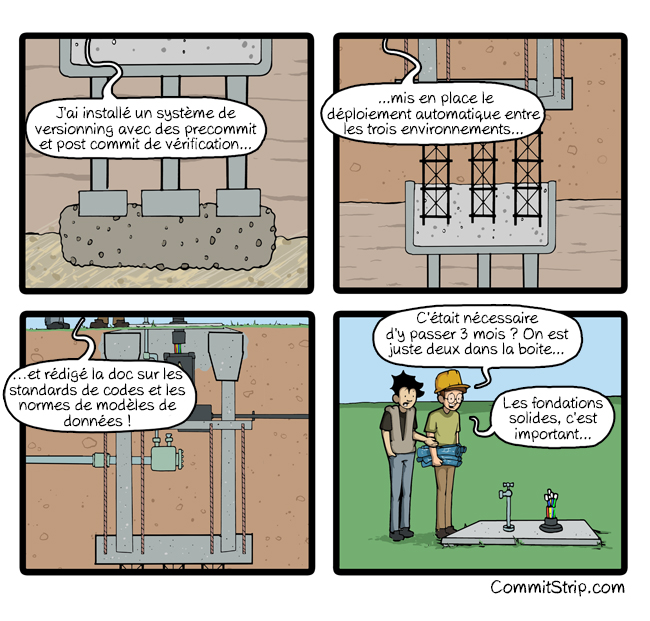
\includegraphics[width=0.8\textwidth]{assets/foundation.jpg}
\caption{Métaphore des bonnes pratiques de développement}
\label{fig:my_label}
\end{figure}